
For this project and according to the research questions, we will be using four models.
\begin{enumerate}
	\item An \textbf{entity model}, which will be a model of the domain concepts. The patient, the different methods for discovering and measuring symptoms. The patient's medical condition and the procedures done to manage the patient's medical condition.
	\item A \textbf{workflow model}, which describes the different processes in a clinical encounter. This will be the flow of the guideline itself at an abstract level.
	\item A \textbf{game model} which will contain the game elements. That means the questions, distractions, answer keys, answer key explanations, rewards and penalties for the different answer alternatives, as well ass passing conditions for the different difficulty levels.
	\item A \textbf{student's learning model} for the student's learning progression.
\end{enumerate}

Models are good for sketches, where we can easily discuss with team members, domain experts and possibly stakeholders. The models can hold a detailed specification of the system, as well as we can use models instead of code to develop the system \parencite{Brambilla2017}.

For this project communication is very important, as the developer needs to understand and be able to model the clinical practice guideline and the clinical encounter at a very high detail. The domain expert in medicine needs to be able to verify that the model is correct.

\section{Extracting knowledge from the clinical  practice guidelines}

\section{MDE and meta modelling}
We will be using a Model Driven Engineering (MDE) approach, mainly for the entity and workflow models. In MDE models serves as the key artefacts that drive the development process \parencite{RodriguesdaSilva2015}. A model in this case is an abstraction of a system under study. It is usually a partly and simplified version, where we often need multiple models to better represent and understand it \parencite{RodriguesdaSilva2015}. A domain model is the conceptual model of a field or expertise that we are examining to solve a problem \parencite{Brambilla2017}.

A metamodel is a further abstraction of a model, which highlights properties of the model \parencite{Brambilla2017}. In figure \ref{fig:Metamodelling} we see that moving up through the levels is an abstraction of the previous model. While moving downward, we are making instantiations of the previous metamodels. With metamodels we can define new languages, as well as defining new properties or features of the available information \parencite{Brambilla2017}. This allows us to make Domain Specific Languages (DSL), which is designes specifically for a specific domain and context \parencite{Brambilla2017}\parencite{RodriguesdaSilva2015}. By using DSLs, we can develop more expressive models, which can enhance communication with or be used by domain experts. 

\begin{figure}[h!]
	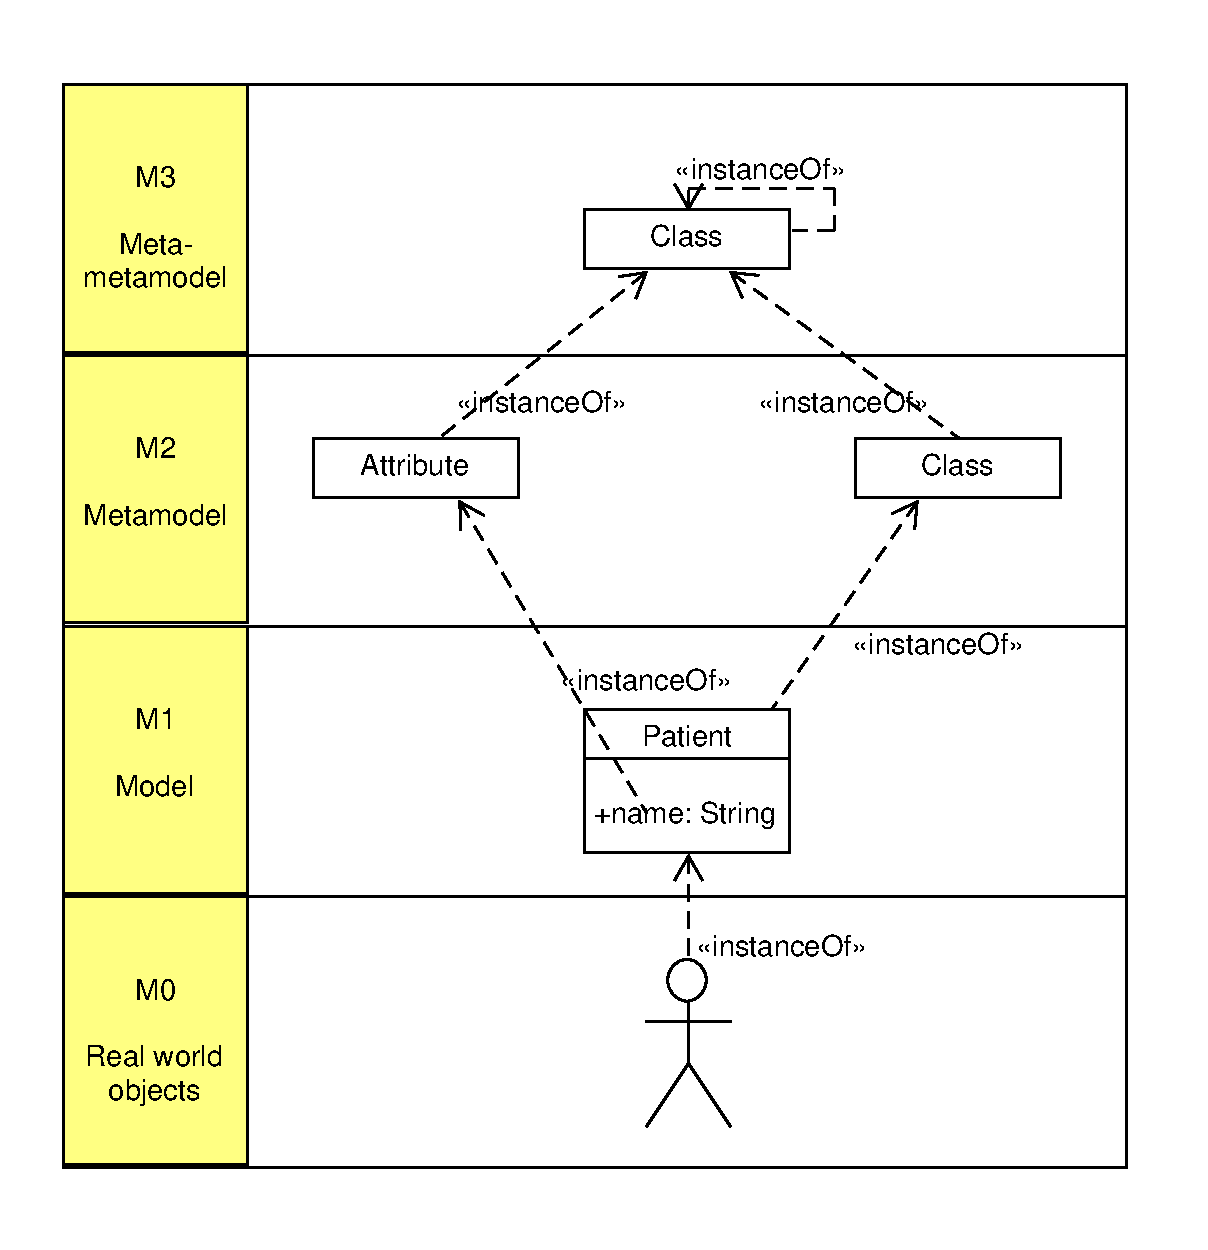
\includegraphics[scale=0.5]{Metamodelling}
	\caption{Metamodeling from a meta-metamodel to a real world object. Derived from \parencite{Brambilla2017}}
	\label{fig:Metamodelling}
\end{figure}

% Say something about how the graph is implemented and a reference to the book.
\section{DPF}
For the enitity- and workflow models, we use a formal diagrammatic approach to model driven engineering, which is called Diagram Predicate Framework (PDF). In software engineering, diagrams are data structures based on graphs. A graph is a collection of vertices, which may be connected by edges.

A definition for DPF is given by \textcite{Rutle2010}: "in DPF, models are represented by a diagrammatic specification \(\mathfrak{S} = ({\mathcal{S}}, C^{\mathfrak{S}} : \Sigma)\). It consists of a graph \(\mathcal{S}\) and set of constraints \(C^{\mathfrak{S}}\) specified by a signature constraint $\Sigma$ ". To simplify the definition to how it is used in this thesis, the models and initiations are represented and implemented using graphs and a set of constraints. The following sections will discuss these graphs in detail.


\textcolor{purple}{TODO Yngve: Why DPF, why not fHIR?}
\section{Entity model}
\textcolor{purple}{TODO Yngve: Explain the main entities in the entity model here}
We will now present the entity model by showing an excerpt, hiding away the details. This will let us easier focus on the concepts and the flow, as the model itself is quite large and complex. See figure \ref{fig:EntityGraphExcerpt}

The entity graph stores information about a specific patient at a certain point of time in the clinical encounter. The patient comes to the emergency clinic. He has some symptoms which the clinician needs to uncover, by doing examinations and asking questions about the patients conditions. What the patient or caregiver tells is modelled as history, while quick examinations such as listening to the chest, looking at the skin, count the number of breaths per minute are modelled in the examination vertex. In some cases the clinician wants to run medical tests which require more time and resources, such as MRI scan, spirometry or blood tests. These tests are modelled as investigations.

Based on the the symptoms collected in history, examination and investigation, the clinician will set a diagnosis. The procedures for what to do with a patient with a given diagnosis is modelled under management. Hospitalization is to change the patients status to outpatient, or inpatient if he is admitted into the hospital. He might need some medication or be given advise for how he should deal with his condition the in every day life. Here the model can be expanded with routines found in other guidelines, we have identified surgery as an example. 

\begin{figure}[h!]
	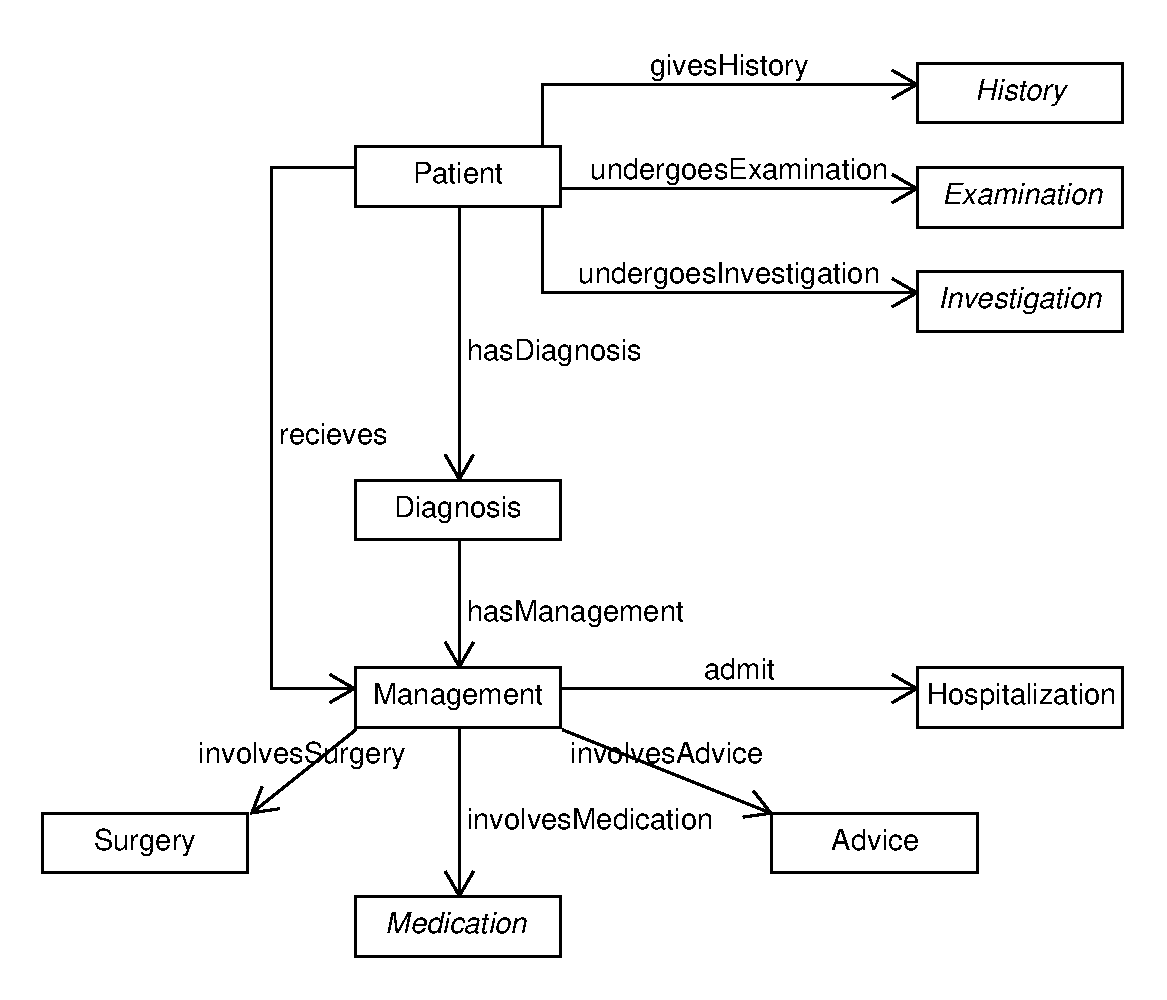
\includegraphics[scale=0.6]{EntityGraphExcerpt}
	\caption {An excerpt of the entity graph. Entity graph represents a patient at a certain point in the clinical encounter}
	\label{fig:EntityGraphExcerpt}
\end{figure}

In figure \ref{fig:EntityGraphPatientDiagnosis} we have expanded the Patient and Diagnosis vertices to reveal more details. PatientName and Gender, identifies the patient with a name and gender. These attributes are important when presenting a patient and his condition in a narrative or scenario. By using a name, it is easier for the reader to see that this is the same patient in different stages of the clinical encounter.

A diagnosis has a name. In the paediatric possible asthma guideline \parencite{RepublicofKeny2016}, the diagnosis has a severity. A lot of medical conditions doesn't have a severity, or they are classified in another way. Here we add multiplicity to the edge which specifies this requirement. 

\begin{figure}[h!]
	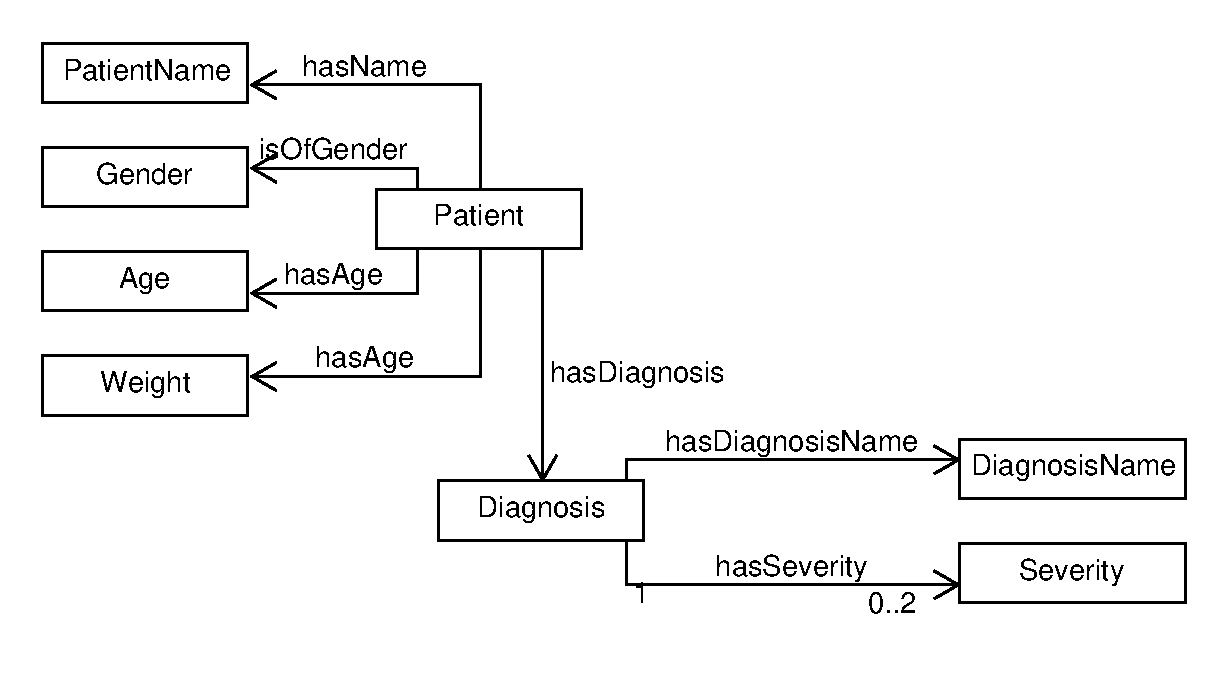
\includegraphics[scale=0.6]{EntityGraphPatientDiagnosis}
	\caption {Showing the details of the Patient and Diagnosis vertices of the entity graph}
	\label{fig:EntityGraphPatientDiagnosis}
\end{figure}

In figure \ref{fig:EntityGraphHistory} we have shown our implementation of the History vertex from figure \ref{fig:EntityGraphExcerpt}. History is what the patient or the caregiver tells about the patient's condition. In the paediatric possible asthma guideline \parencite{RepublicofKeny2016} we have identified three symptoms which the clinician can ask the patient or the caregiver about. Here we introduce inheritance, where the specific symptoms inherits the examination vertex. Each symptom the patient or caregiver tell about, will have a measurement. In this specific case, all the history symptoms are boolean. Either they have the symptom or they don't. The symptom values inherits from a Measurement vertex.

\begin{figure}[h!]
	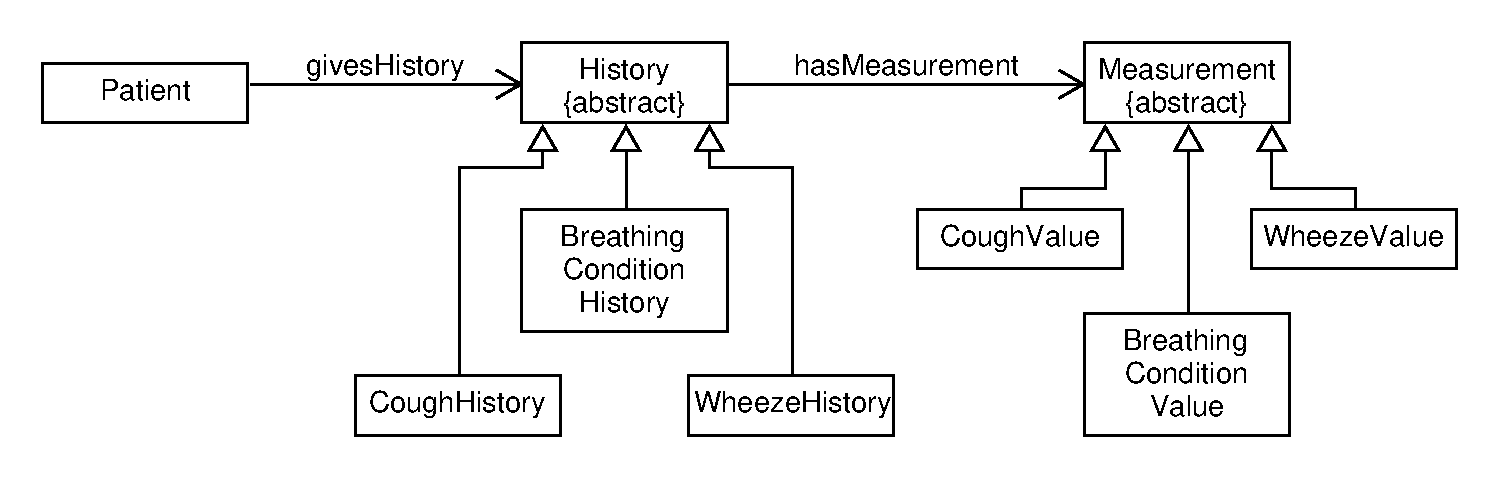
\includegraphics[scale=0.5]{EntityGraphHistory}
	\caption {Showing the implementation of History in the entity graph. What the patient or caregiver tell about the patient's condition}
		\label{fig:EntityGraphHistory}
\end{figure}

For Examination we follow the same principles as History. We implement it by letting each symptom inherit an Examination vertex. Each symptom has value which inherits from a Measurement vertex. In figure \ref{fig:EntityGraphExamination} we have shown the inheritances for each vertex with one arrow and a box. This is of practical reasons when drawing, as there are so many symptoms and it will be confusing to draw an arrow for each of them. Here the values which are stored are a bit more mixed than for History. Consciousness is measured using an AVPU scale, where A is the patient is Alert, V is Verbal, P is responding to pain and U unconscious. These are enumerates, where we store either A, V, P or U. Pulse Rate, Respiratory Rate, Oxygen Saturation are all numerical values. The other symptoms are registered as boolean values. Keep in mind that Jaundice is really not a part of the paediatric possible asthma guideline \parencite{RepublicofKeny2016}. It is included as part of the antibiotic treatment.


The implementation of Investigation would be just as we did with History and Examination. For asthma they use a lab test called spirometry, but it is not included in the paediatric possible asthma guideline \parencite{RepublicofKeny2016}, so we don't include it in our model

\begin{figure}[h!]
	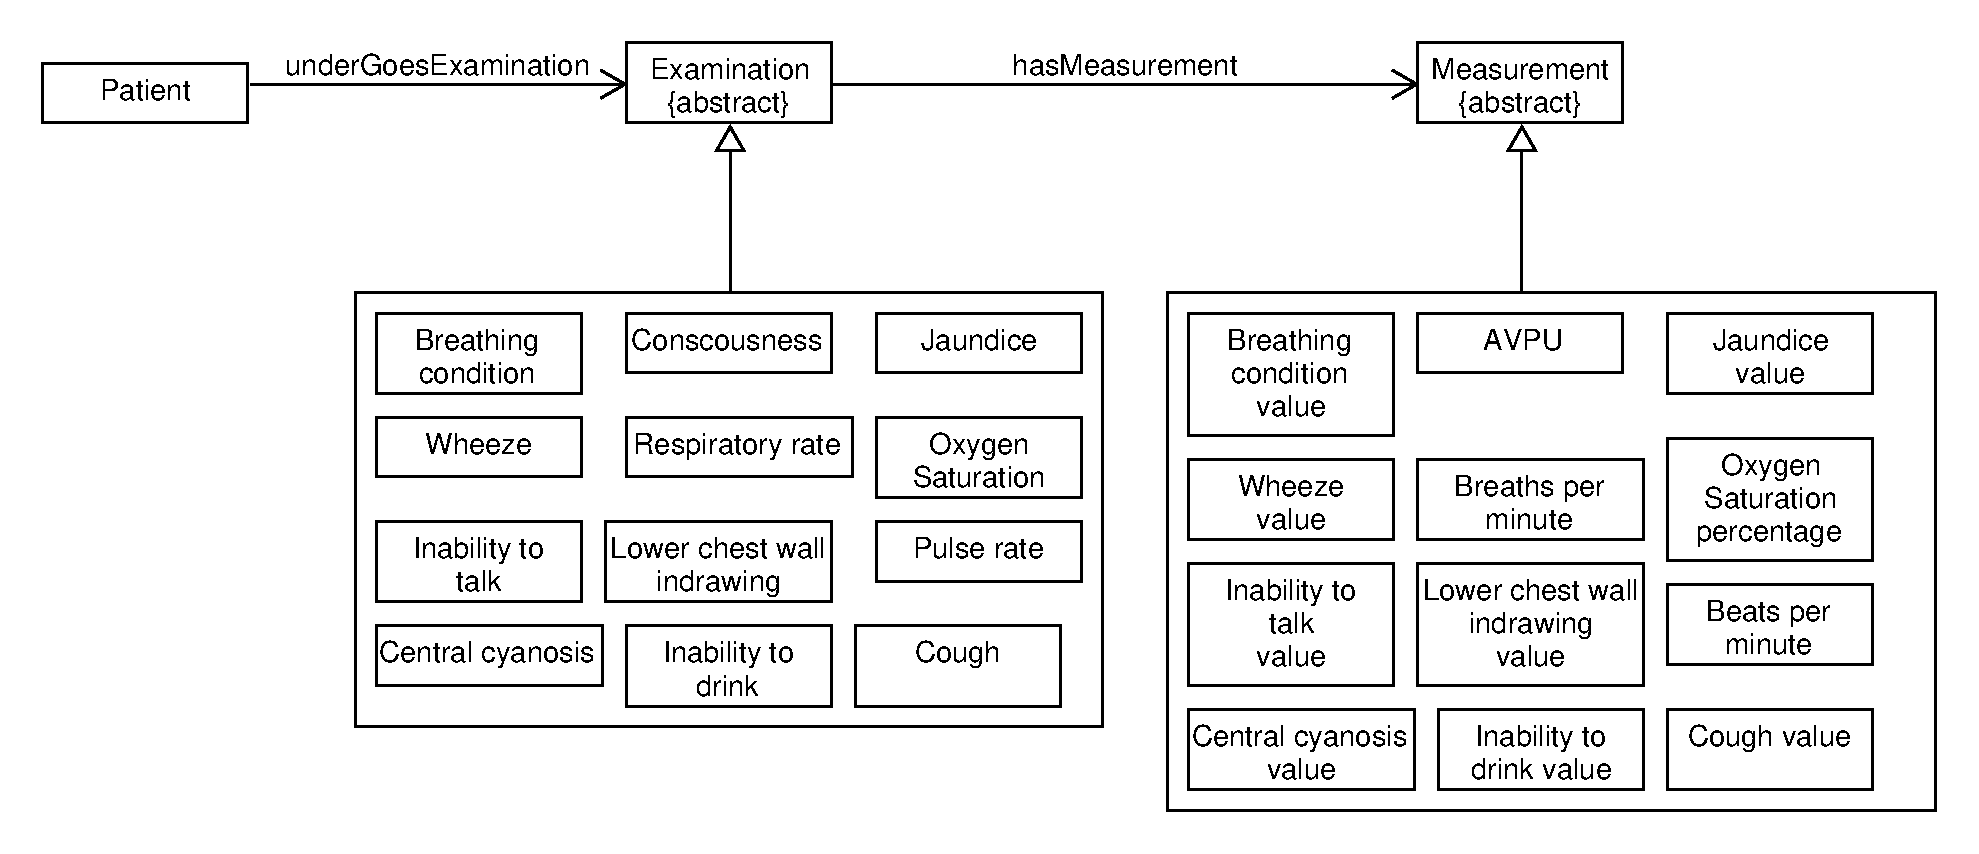
\includegraphics[scale=0.4]{EntityGraphExamination}
	\caption {Showing the implementation of Examination in the entity graph. What symptoms the clinician can observe the patient has}
	\label{fig:EntityGraphExamination}
\end{figure}

In the paediatric possible asthma guideline \parencite{RepublicofKeny2016}, there are used five medications to treat the patient, as well as antibiotics which is a class of medications. We will talk about each medicine in the model as there are some details which needs to be clarified. See figure \ref{fig:EntityGraphMedication}.


\begin{itemize}
	\item \textbf{Oxygen} is a medication, which is given to patient which doesn't get enough oxygen by breathing. In asthma this happens because of the airways are tightened. The paediatric possible asthma guideline \parencite{RepublicofKeny2016} doesn't specify how the oxygen should be administered, but the paediatric guidelines contain a guideline for prescribing oxygen\parencite{RepublicofKeny2016}. We have decided to model a part of the prescribing oxygen guideline, to be able to ask simple control questions to verify that the student still remembers how to administer it. Oxygen has a route, which is inhaled. The method is oxygen face mask with reservoir bag. The rate will be given in litres per minute. The duration of the treatment will be until the oxygen saturation is at a high enough level.
	
	\item For \textbf{antibiotics}, the CPG says the antibiotic should be given according to the paediatric pneumonia guideline \parencite{RepublicofKeny2016}. We have decided to include the antibiotic treatment in detail in the model, but we have also kept Antibiotic as a medication, such that we later can ask a question where we don't go in more detail than just antibiotic, which is the detail level of paediatric possible asthma guideline \parencite{RepublicofKeny2016}. The antibiotic treatment consists of two medications gentamicin and penicillin. Gentamicin and penicillin are given as an injection either intramuscularly or intravenously, which is modelled as Route and Method. The rate is given by iu per kg, mg per kg, per 6hours or per 24 hours. If the patient has jaundice, he shouldn't be given penicillin. How much penicillin and gentamicin will be given according to the patient's weight.
	
	\item \textbf{Prednisolone} is a steroid used to calm and prevent inflammation in the airways. The clinician will administer a dosage calculated by the patient's weight. There is a max dosage per day, and the age will determine how high that max dosage is. The rate is given in mg per day. The duration is 3-5 days. The route is oral and the form is tablet. In situations where prednisolone needs to be given more than 5 days, it will be administered with the route inhaled and form inhaler.
	
	\item \textbf{Corticosteroid} is another steroid, which is given to in scenarios of recurrence asthma symptoms. The CPG specifies that corticosteroid should be inhaled. This is represented in the model by the Route vertex. The method the which will be used to inhale corticosteroid is represented by the Form-vertex. The Form is MDI with spacer, preferably with spacer with face mask. 
	
	\item \textbf{Salbutamol} is inhaled to open the airways of an asthma patient. The Rate vertex tells at which rate the patient should be taking salbutamol. Asthma patient is given salbutamol at a rate of 2.5mg per 20 minutes if nebulized, or 6 puffs per 20 minute if the inhaler is used. The Duration is up to one hour or three doses if needed. The method is inhaled and the form is either nebulizer or inhaler.
	
	\item \textbf{Ipratropium bromide} is modelled much like salbutamol with a Rate and a Duration. The rate is given in mcg every 20 minutes for a duration of one hour if needed. The route is inhaled and the form is inhaler.
\end{itemize}

 We have kept the Dosage vertex, while it is not in use. It can be used to represent the total amount of a specific medication given to the patient during this treatment.
 

\begin{figure}[h!]
	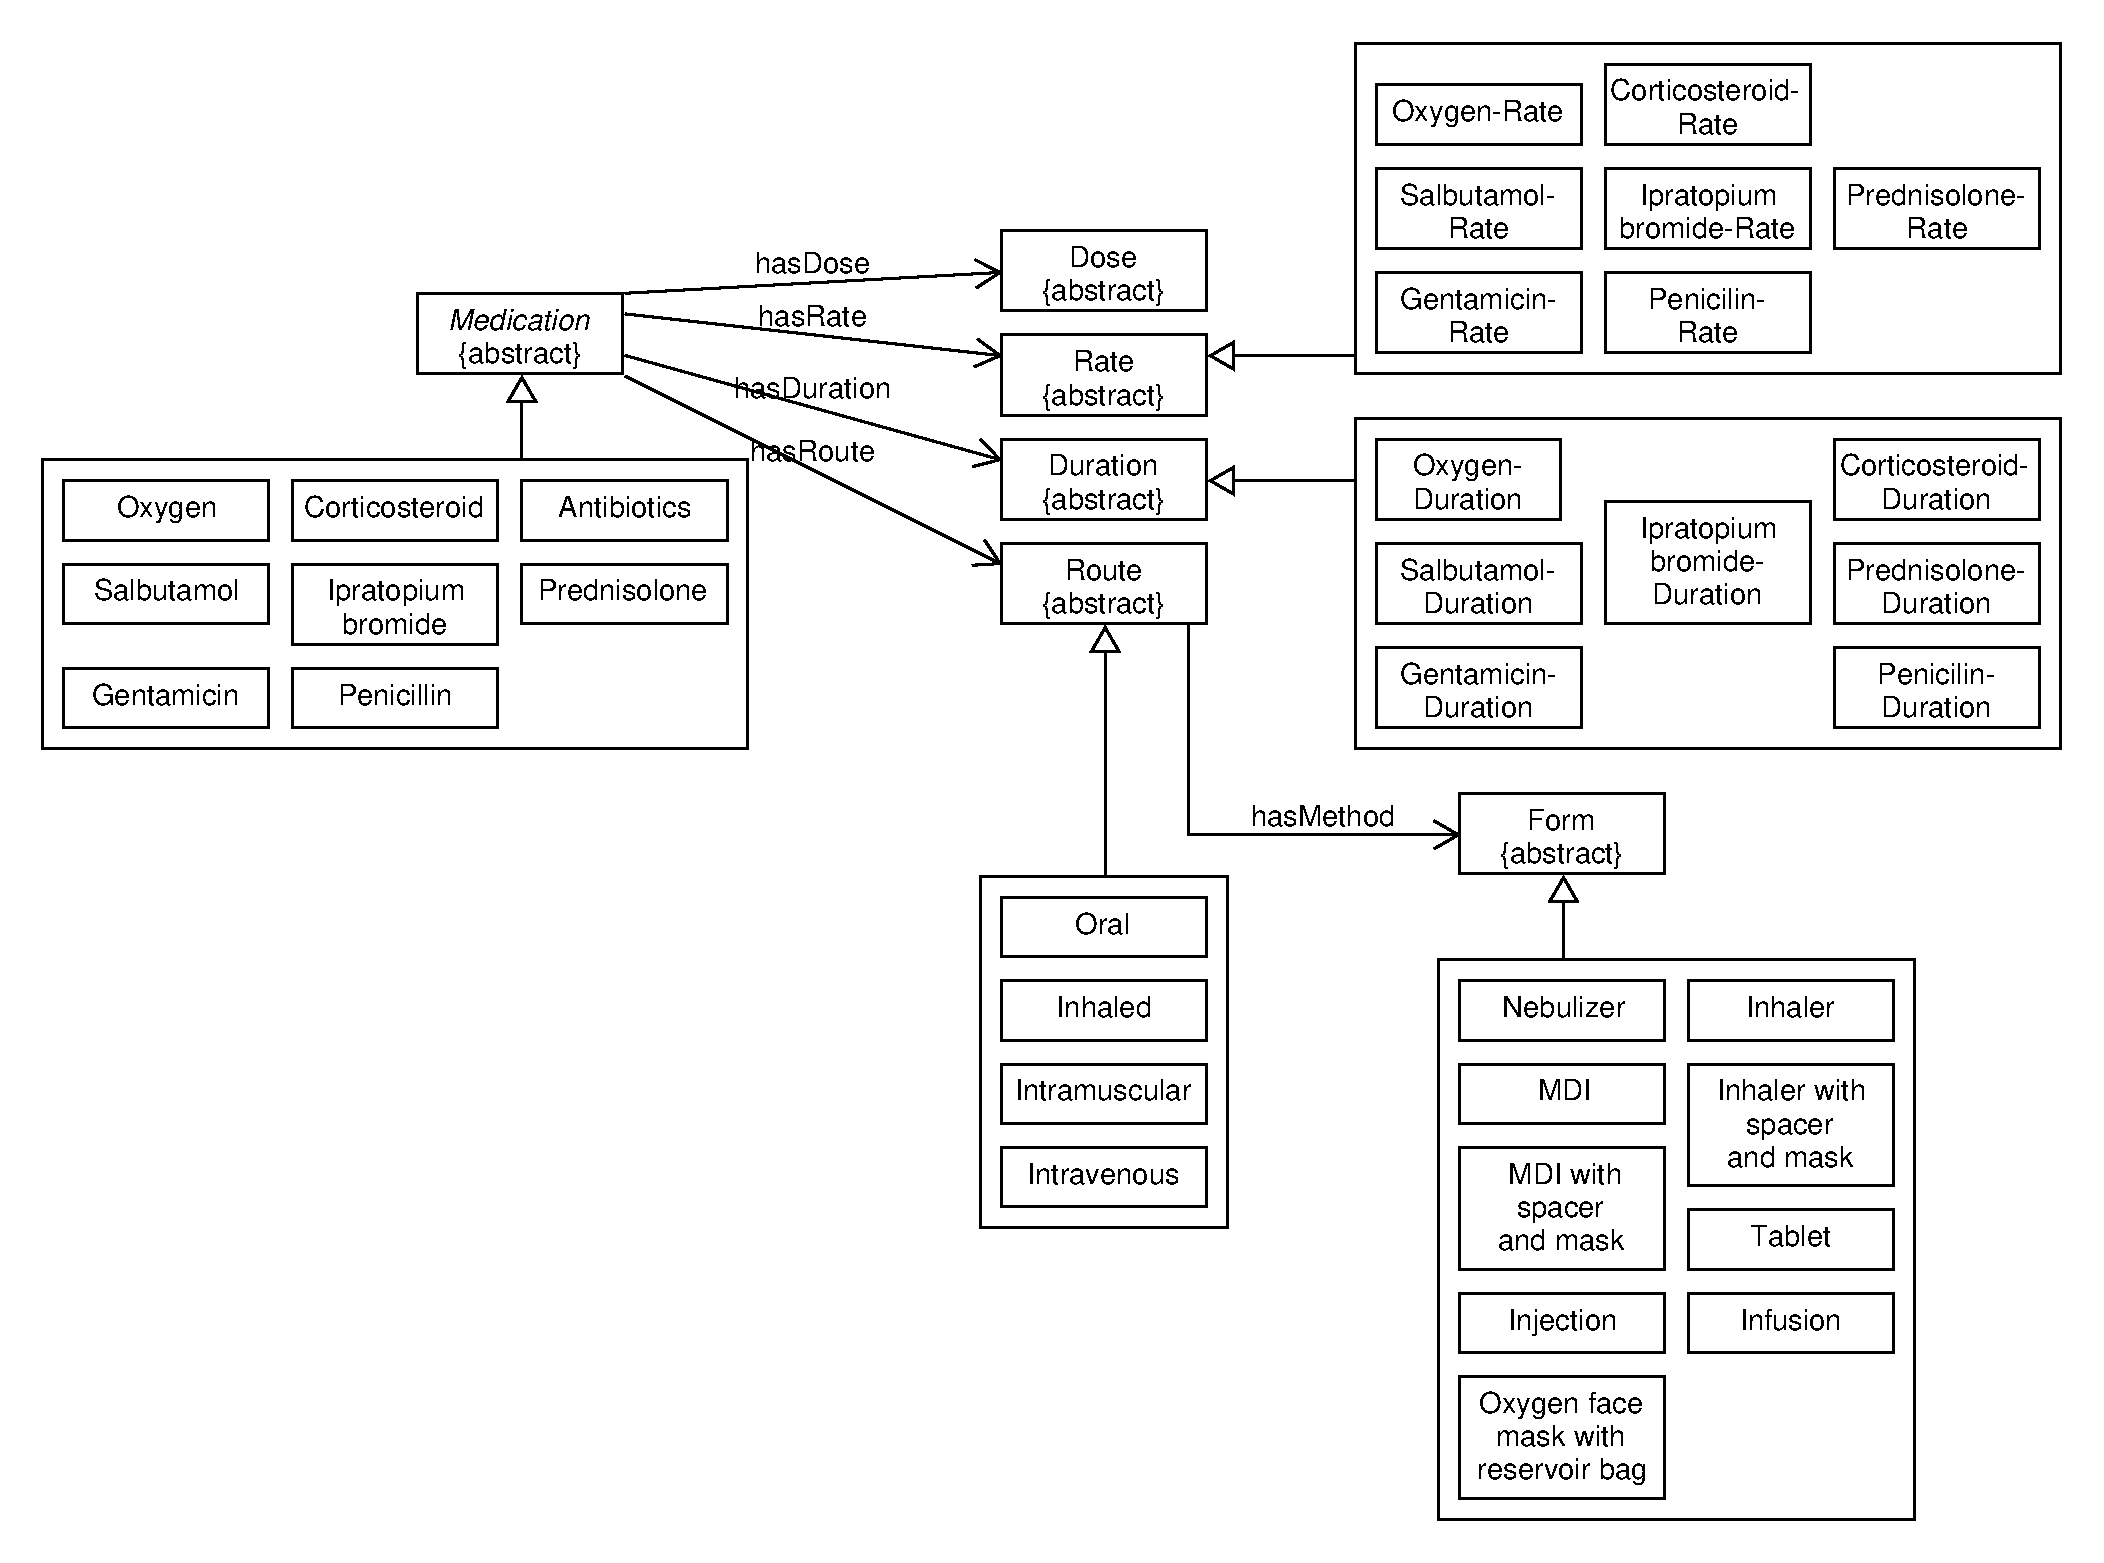
\includegraphics[scale=0.38]{EntityGraphMedication}
	\caption {Showing the implementation of Medication in the entity graph. How to administer a medication to patient}
	\label{fig:EntityGraphMedication}
\end{figure}

 Another detail must be clarified when implementing instances of the medications. The route must be given names which can be uniquely identified for each medication. An example is Ipratopium Bromide and Salbutamol which both uses the Route Inhaled. Ipratopium Bromide uses only the inhaler, while Salbutamol can be given using the nebulizer. If Ipratopium Bromide is sharing the same Inhaled vertex as Salbutamol during instantiation, it will look like Ipratopum Bromide can be nebulized. By creating a new instantiation of Route per medication, and uniquely identify them by name Inhaled1, Inhaled2 or InhaledSalbutamol, InhaledIpratopium, we avoid this problem. Now we can connect Salbutamol with Inhaled1 and have edges to Form Inhaler and Nebulizer. Ipratopium Bromide has an edge to Inhaled2, which has an edge to Inhaler. Then we have an instantiation where Ipratopium Bromide can only be inhaled using the Inhaler. See figure \ref{fig:RouteMethodProblem}.


\begin{figure}[h!]
	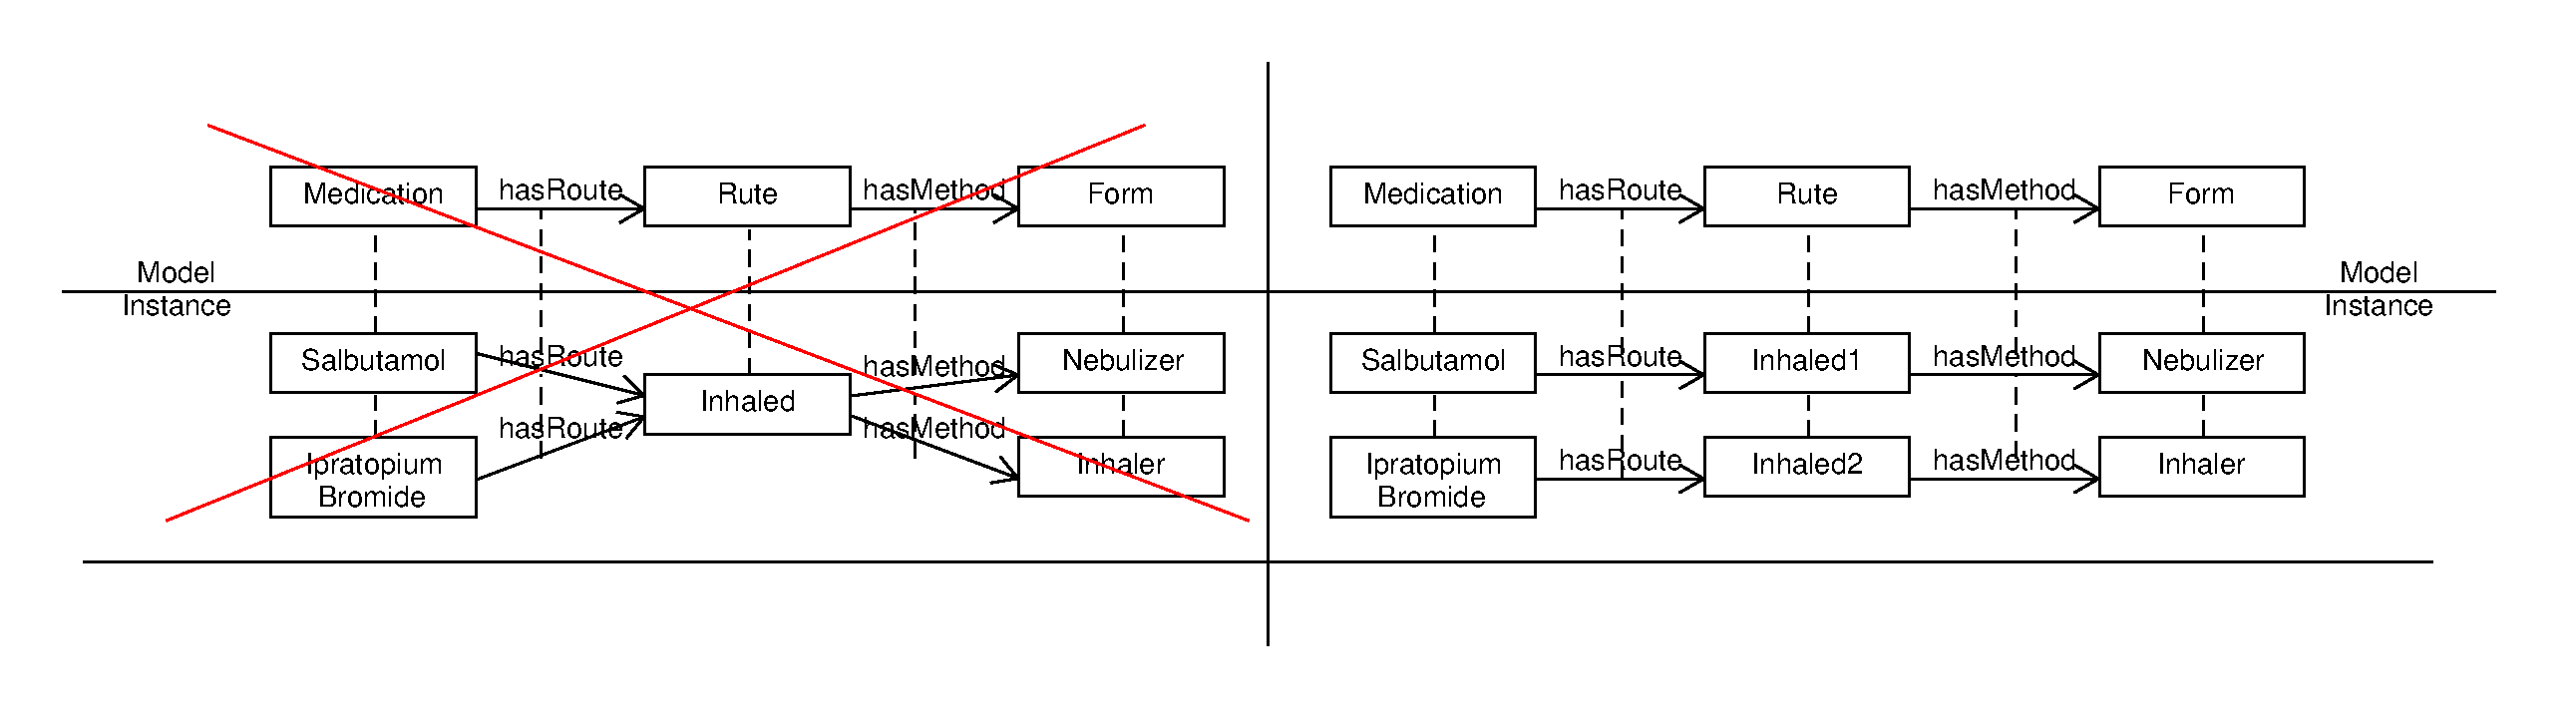
\includegraphics[scale=0.3]{RouteMethodProblem}
	\caption {To the left we don't know which medication has been inhaled using the nebulizer or inhaler. To the right we have specified this in the instantiation, by using two Inhaled-vertices and uniquely identifying them by giving them different names}
		\label{fig:RouteMethodProblem}
\end{figure}

\subsection{Generic entity model}
In the previous section, we had the focus on developing a specific entity model for the paediatric guideline of possible asthma \parencite{RepublicofKeny2016}. In fact by introducing inheritance, we actually made a specific and a generic model. In the model, we use the keyword \{abstract\} to note an abstracted vertex. The inheriting vertices become the specifications of the abstract vertex. 

In figure \ref{fig:GeneralEntityGraph} we have showed the the generic model. It only shows the abstracted vertices and not the specifications. A specific entity model for a specific guideline, will show both the abstractions and the specifications of them. The specifications need to be adapted for that specific guideline, and can not use the same as for paediatric guideline of possible asthma \parencite{RepublicofKeny2016}.

\begin{figure}[h!]
	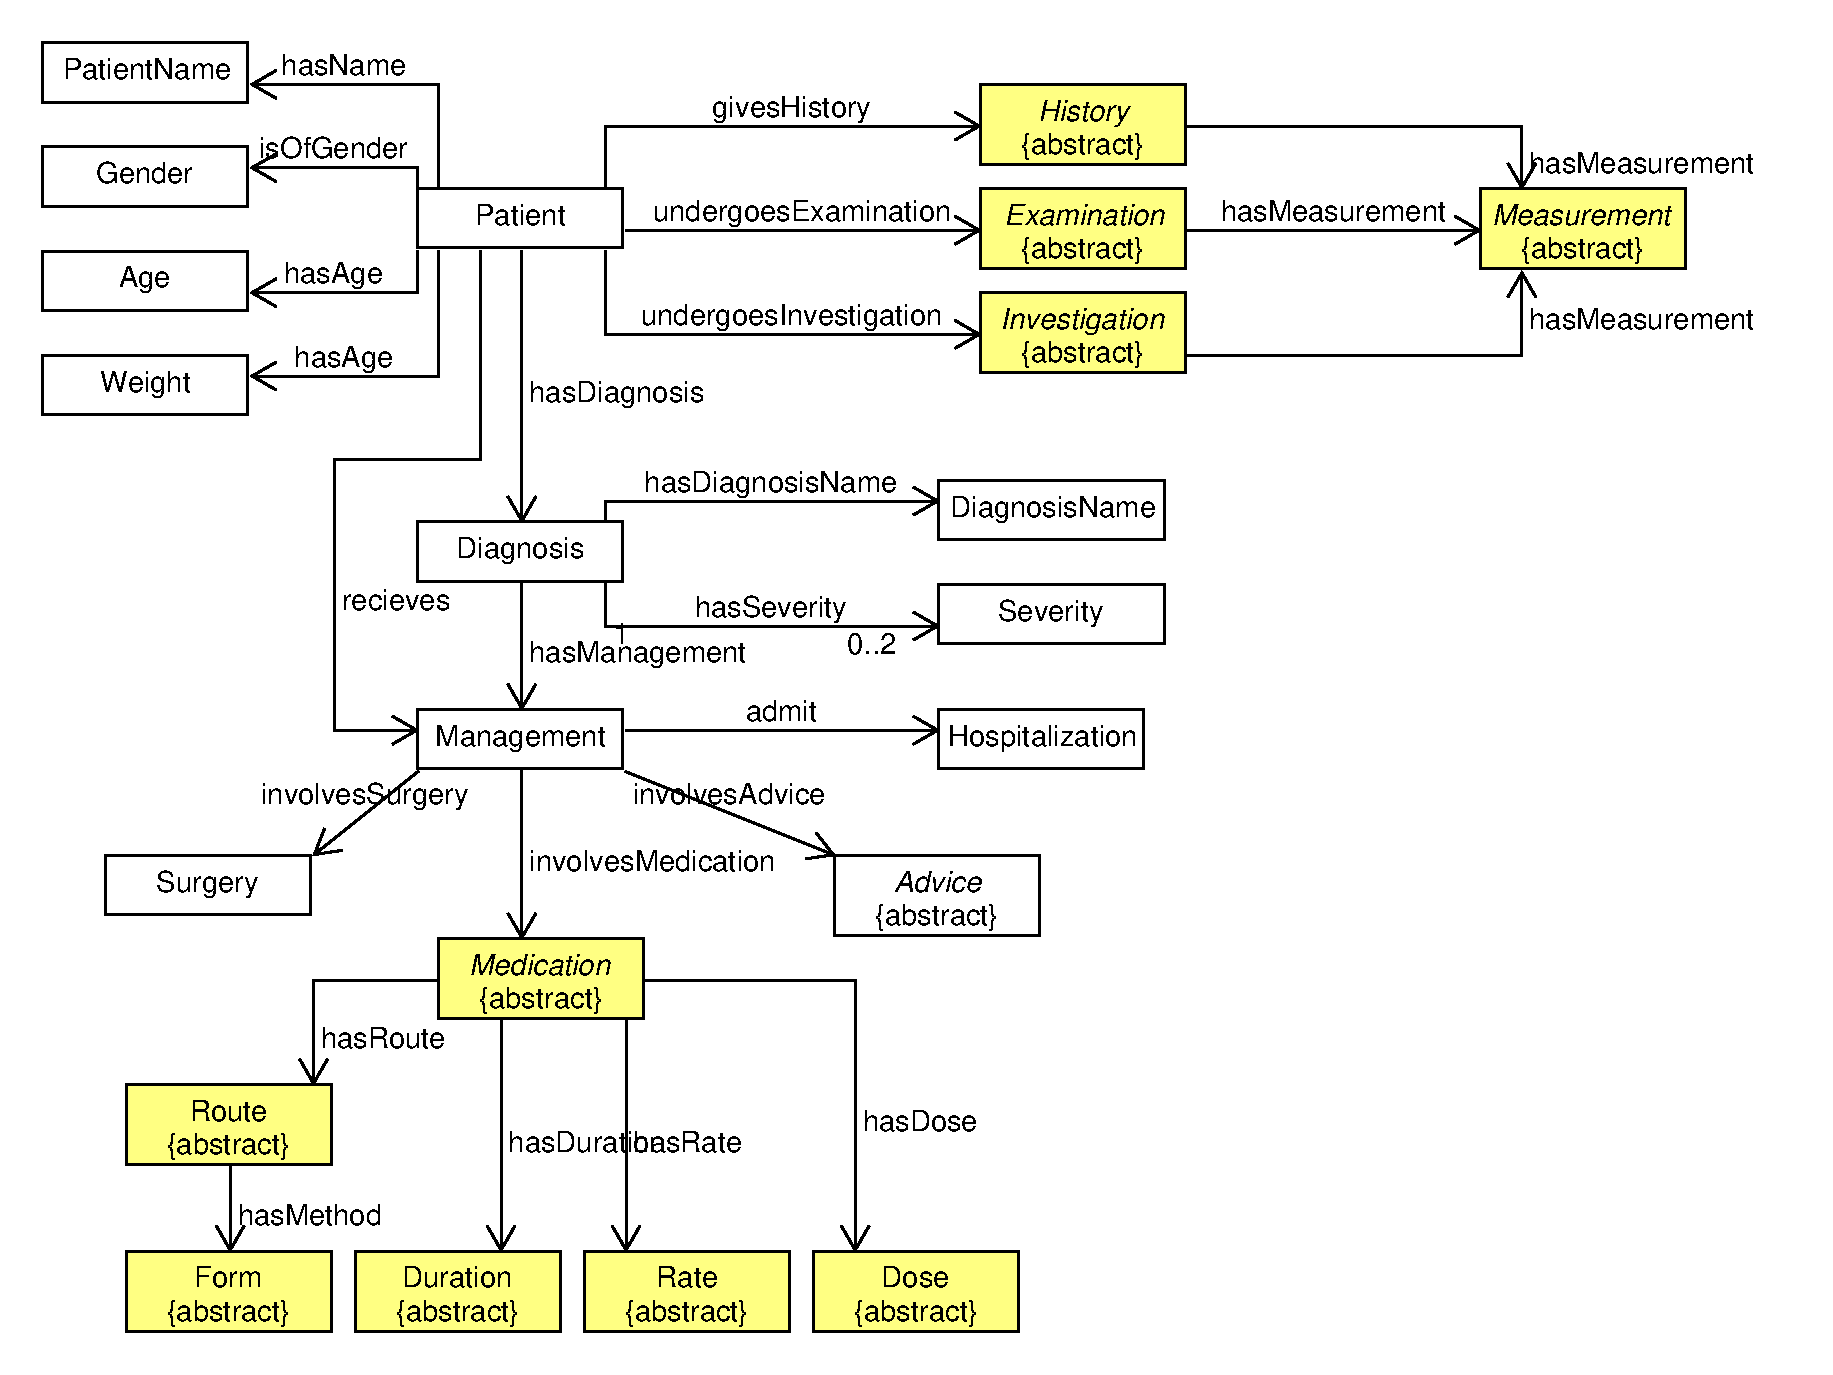
\includegraphics[scale=0.4]{GeneralEntityGraph}
	\caption {A generic entity graph contains abstractions. An entity graph for a specific guideline, contains specifications for those abstractions. Yellow boxes indicate specifications we have shown for paediatric guideline of possible asthma \parencite{RepublicofKeny2016}}
	\label{fig:GeneralEntityGraph}
\end{figure}

\section{Workflow model}
We model the dynamics of clinical encounters with a workflow model. The clinician starts with the assessment, where he examine the patient and listen to what the patient and the caregiver has to say about the the patient's condition. The clinician starts to get an idea of what condition the patient may suffer from. The clinician continues with the diagnostic part, where he asks more targeted questions to the patient and caregivers about the condition, do more of the examination and perhaps order lab tests as part of the investigation. This process can strengthen the clinician's assumptions about the condition, and he may be able to set a specific diagnosis.

The next step is the management and treatment. This can be changing the patient's status from outpatient to inpatient, do surgery, medication, physiotherapy, cognitive behavioural therapy or other forms of treatment. The treatment may be done in iterations or repeated.


The final step is to evaluate. The treatment may have to be adjusted to get the right effect. The diagnosis has changed. For example the severity of asthma may have changed from severe to mild or moderate after the treatment. Or we have initial set the wrong diagnosis, for example we have treated a patient for possible asthma, but in fact an object was stuck in the airways of the patient.


\begin{figure}[h!]
	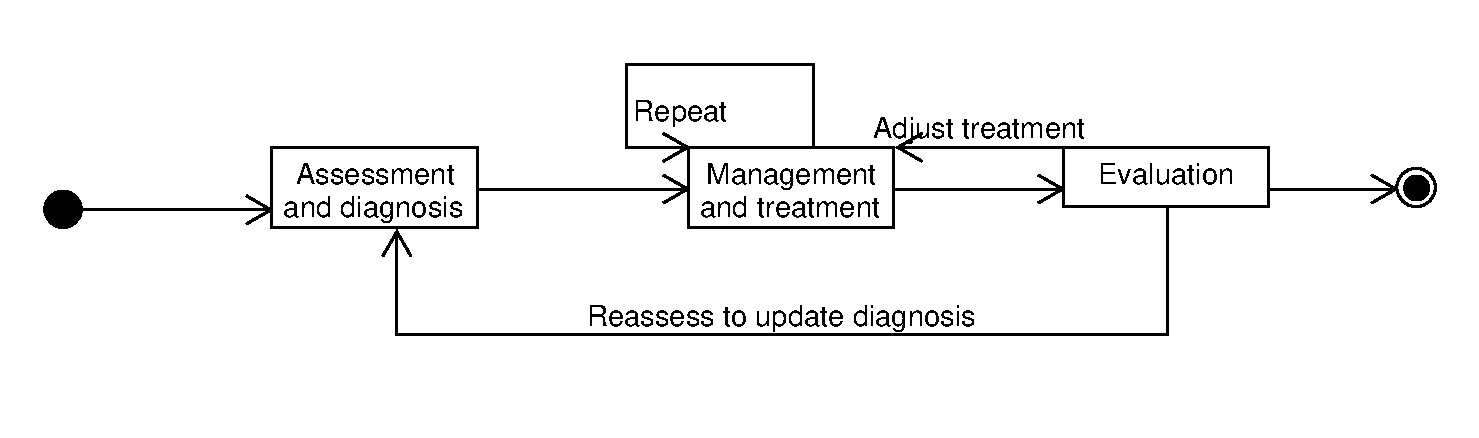
\includegraphics[scale=0.5]{WorkflowGraph}
	\caption {The workflow models is a model of the clinical encounter}
		\label{fig:WorkflowGraph}
\end{figure}

The idea of the workflow model is to describe the process of a clinical encounter. When making scenarios for the game, we know in which order the scenarios should come. The entity model is also connected to the workflow model. When doing a an assessment and diagnosis, you are looking at the examination, history and vertices of the entity model, where the diagnosis vertex answer to what the specific diagnosis is. For doing management and treatment, you look at the vertices under management in the entity model. An evaluation will be done by looking at the examination and investigation vertices to see if the patient has become better. The treatment needs to be adjusted accordingly to the evaluation. If the evaluation says we can't do more for the patient and there's no need for a follow-up, we exit the workflow model.

\textcolor{red}{Should perhaps reference to Rabbis articles here? 
	Coordination	of multiple metamodels, with application	to healthcare systems.
A flexible metamodelling approach for healthcare systems. }

\section{Metamodeling}

\textcolor{red}{I struggle when it comes to talking about MDE, DPF, metamodeling and model transformation, as I lack very basic knowledge about the subjects. Rutle, Rossini, Rabbi are all hard to read}

\textcolor{purple}{TODO: Yngve has a definition of metamodels which aren't so easy to read}

In figure \ref{fig:MetamodelEntityGraph}, we make an instance of the entity model. An instance of the entity model describes an actual patient at one point in the clinical encounter. 

For an instance to be valid, the vertices and edges have to correspond to a part of the model. We demonstrate this by adding dotted arrows in figure \ref{fig:MetamodelEntityGraph}. 

In figure \ref{fig:MetamodelEntityGraph} a patient tells the clinician that he struggles with a wheeze and a cough. Cough and Wheeze inherit from History in the model. Difficulty breathing is part of \ref{fig:EntityGraphHistory}, but is not represented here as the patient hasn't brought up this issue or been asked about it. We see how two inheritances og History translated in the instance from the model. The Measurement vertex holds the measurements of the History vertices. A patient with a wheeze and a cough is diagnosed with asthma, which is shown in the instance.

\begin{figure}[h!]
	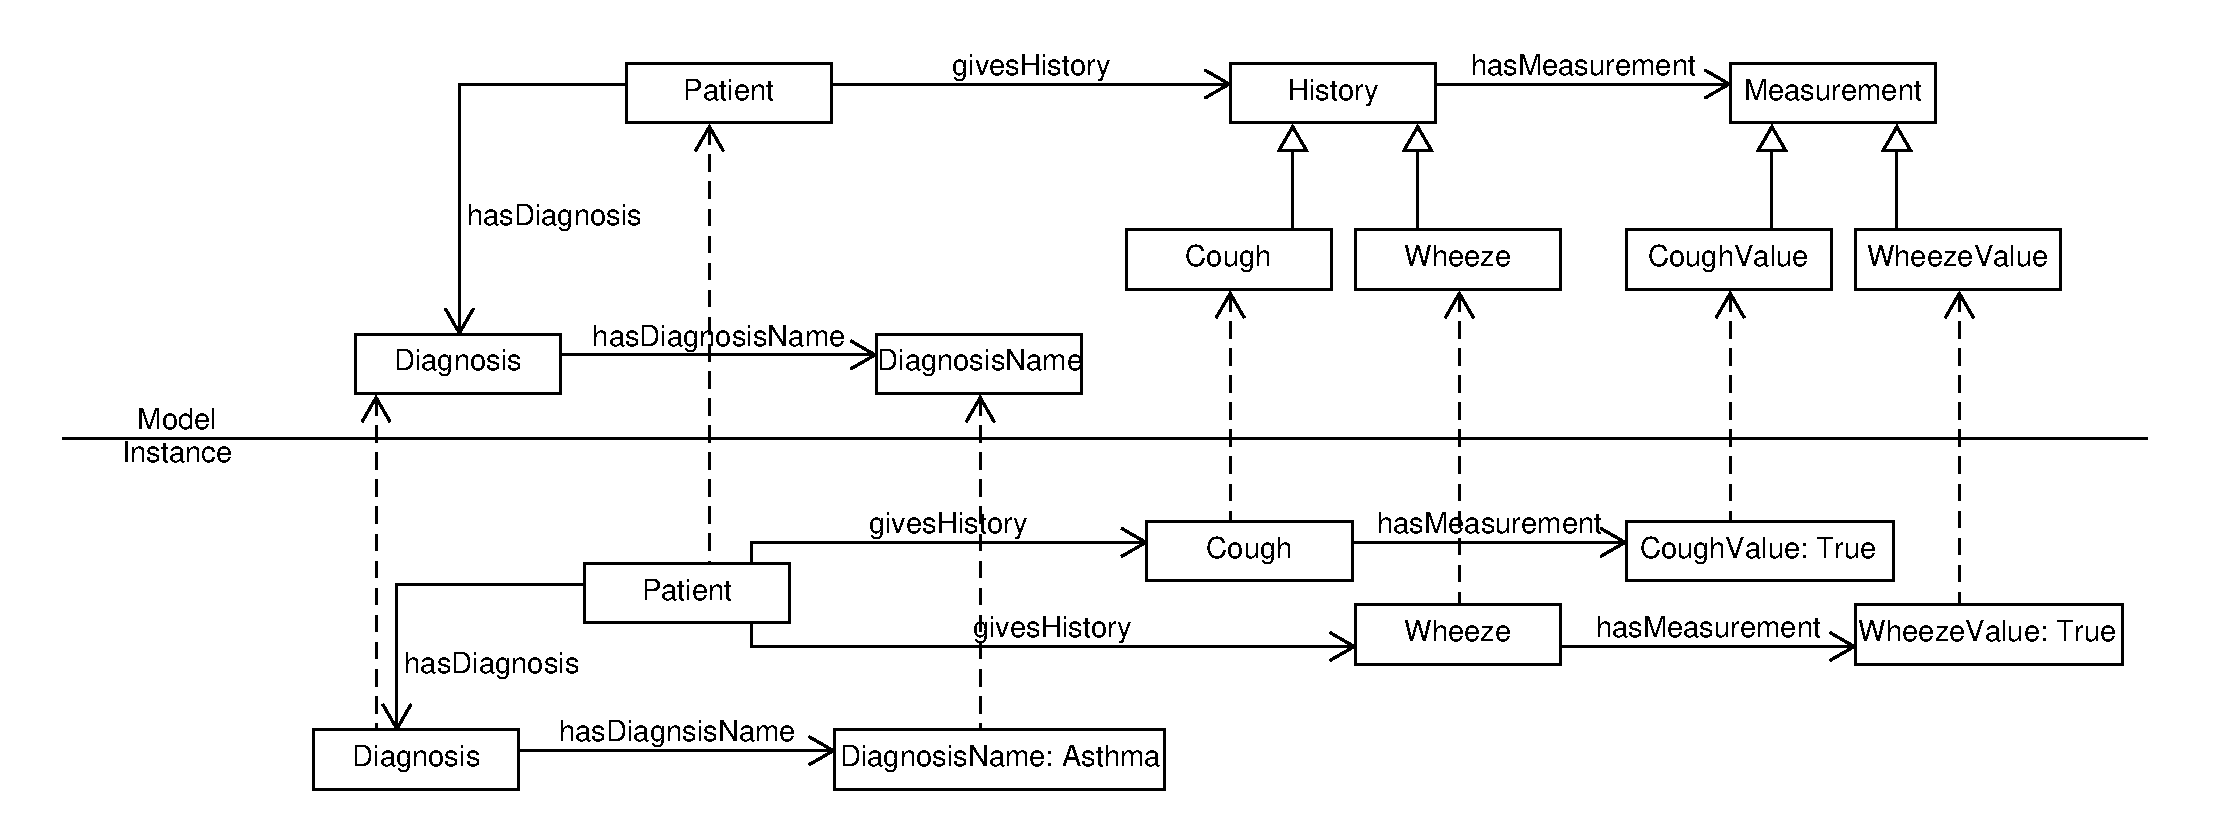
\includegraphics[scale=0.35]{MetamodelEntityGraph}
	\caption {A model and an instance of the entity model. For a valid instance, every vertex and edge in the instance has a corresponding vertex and edge in the model}
		\label{fig:MetamodelEntityGraph}
\end{figure}

\textcolor{purple}{TODO Yngve: shows where you are in guideline figure \ref{fig:MetamodelEntityGraph}}

In figure \ref{fig:IntegratedEntityWorkflowModels} we show a entity instance working together with the workflow model. For the assessment, we look at the History and Examination vertices. For Diagnosis, the DiagnosisName and Severity. Keep in mind that under Diagnosis, the clinician may do further examinations and questions to the patient to confirm his assumption, or which may cause him to think about other diagnosis. Management, the asthma is severe so we change the patient's status to inpatient by updating the Hospitalization vertex. We also look at the Medication vertex under Management. We only care about the medications for now in this example, and not how the medications should be administered. The Evaluation holds a reference to a new entity instance, which holds the updated information about the patient's symptoms. The clinician needs to act accordingly and adjust the treatment.

\begin{figure}[h!]
	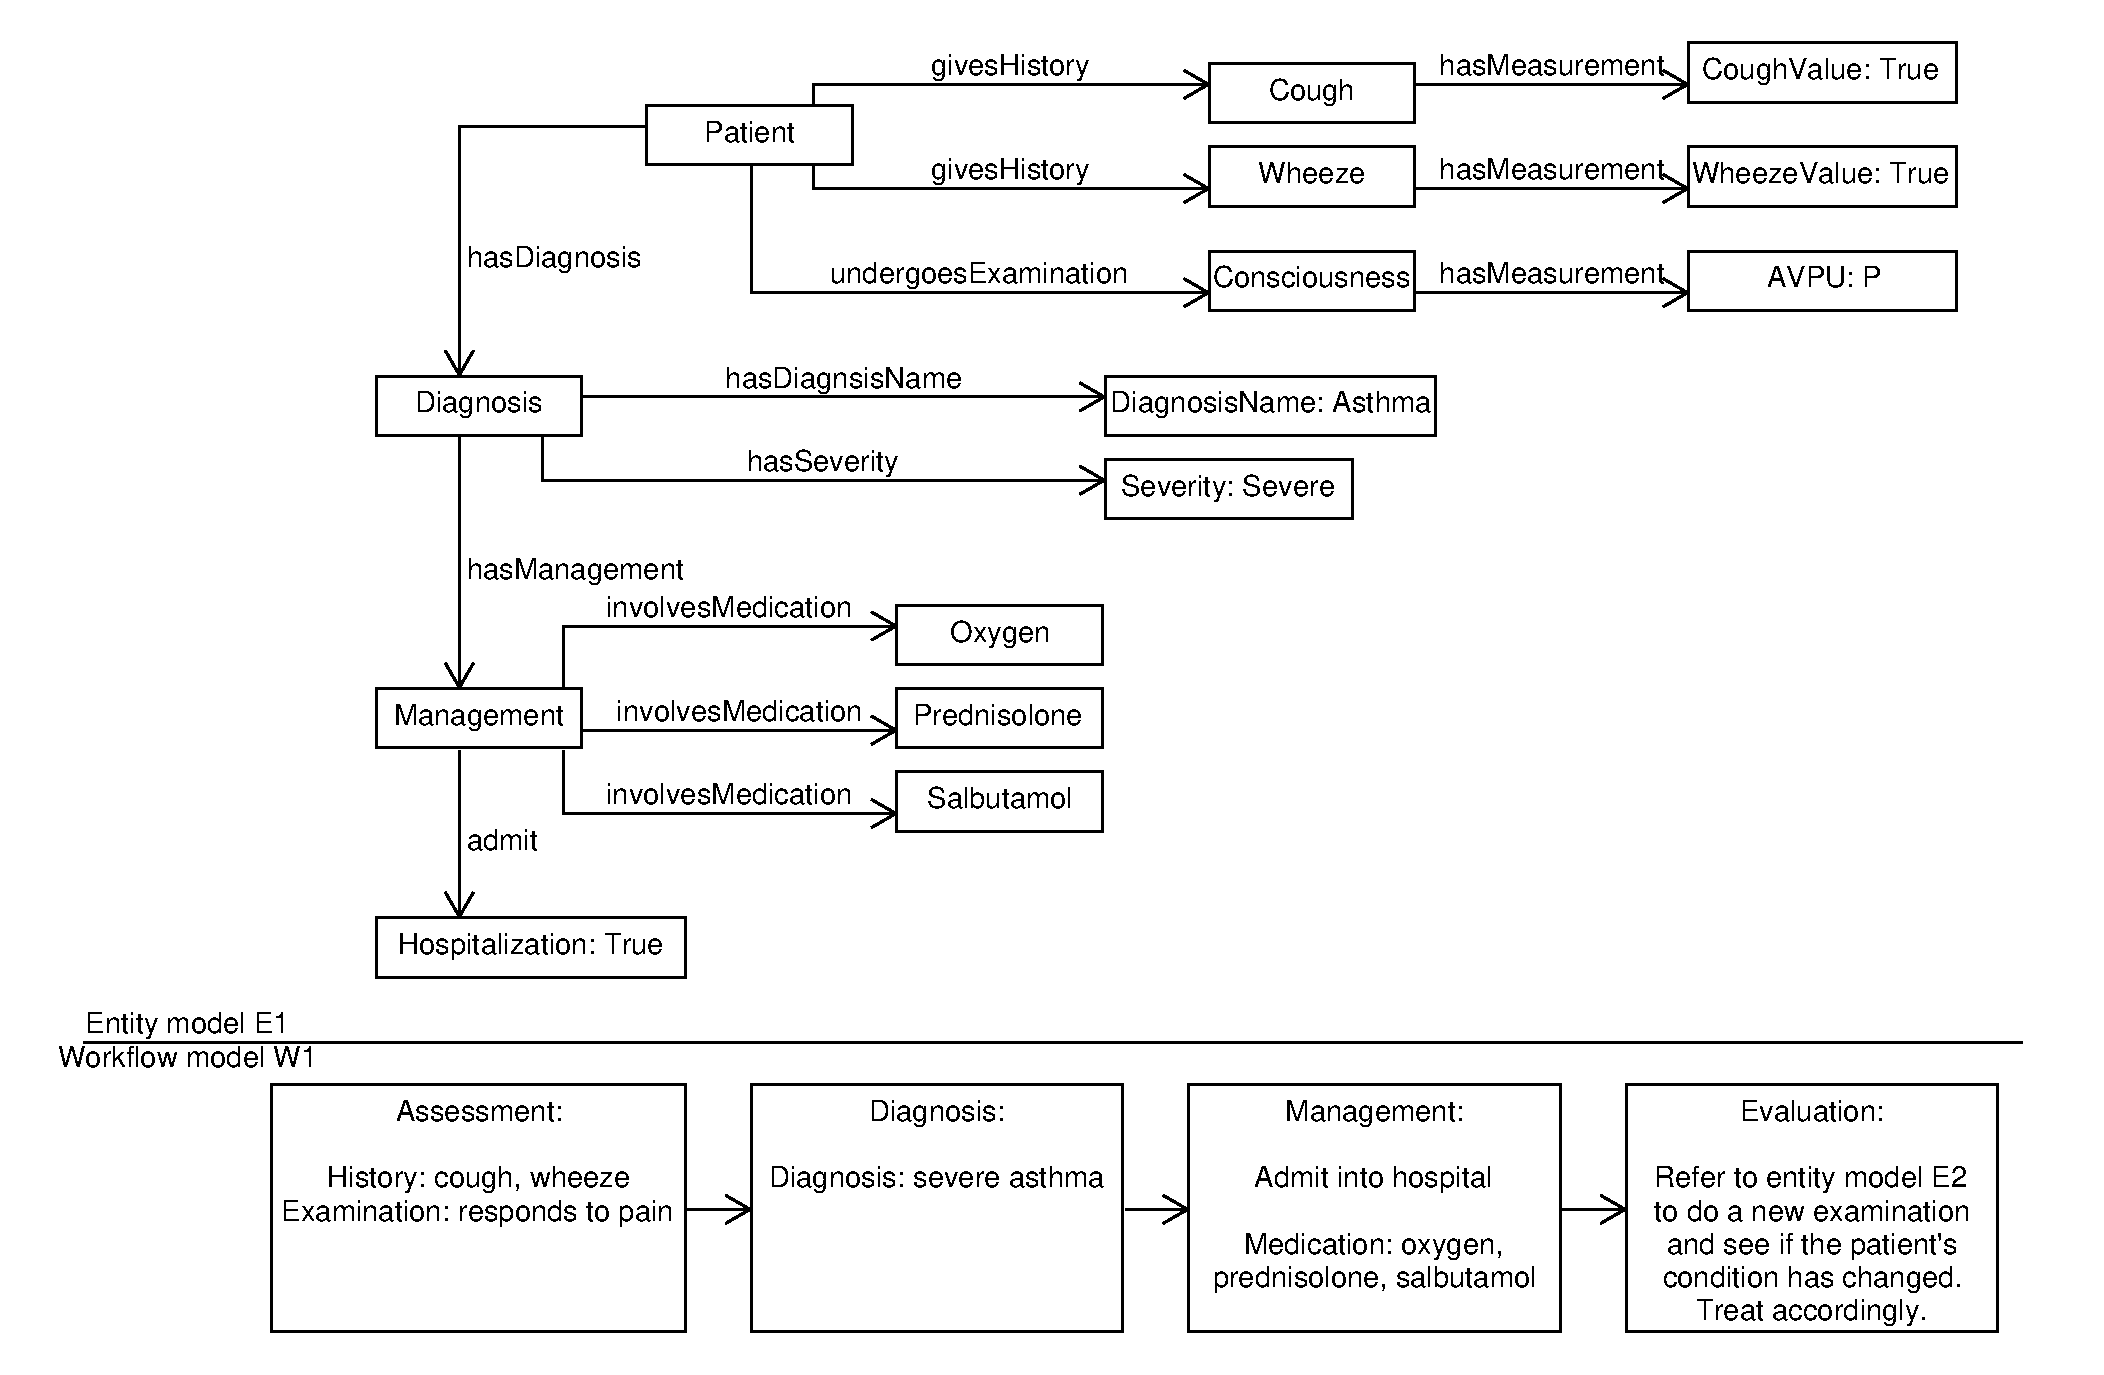
\includegraphics[scale=0.38]{IntegratedEntityWorkflowModels}
		\caption {An instance of the workflow model at the bottom, working together with an instance of the entity model at the top}
		\label{fig:IntegratedEntityWorkflowModels}
\end{figure}


\section{Game model}
The game model is not implemented using DPF and MDE like the entity model and workflow model. However, a MDE game model could be relevant in future work.

Here we will give a brief explanation of the content of the game model. It can work as a reference point for the next chapter, where we will discuss the game elements more thoroughly.
\begin{itemize}
	\item \textbf{Category:} a CPG is written for a specific medical condition. The quiz category will be the medical condition, or the name of the CPG the quiz is written for.
	\item \textbf{Discipline:} a question is written for a specific step in the clinical encounter, which the workflow model is an abstraction of. Discipline is a step in the clinical encounter.
	\item \textbf{Level}: Is the difficulty level of the question.
	\item \textbf{Passing condition:} a condition the student has to fulfil to pass a specific  difficulty level.
	\item \textbf{Required Minimum Skill:} a condition the student has to fulfil to be able to play questions at a specific difficulty level.
	\item\textbf{Entity Instance}: a pointer to an instance of an entity graph. It is used together with a template to generate text.
	\item \textbf{Question:} a pointer to a template model. By using a template model, we can reuse templates on many entity instances.
	\item \textbf{Alternative:} or distraction. It is one of the answer alternatives for a question. 
	\item \textbf{Reward:} a reward or penalty is given based on the correctness of the distraction. A distraction can be degrees of right or wrong, which is reflected by the reward.	
\end{itemize} 

The game model is paired with a template model. By separating the template into its own model, we can reuse the same template for many questions.
\begin{itemize}
	\item \textbf{Narrative:} template which represents a question. The template contains tags which points to vertices in an entity graph. When the template is paired with an instance of such a graph, it will produce a textual presentation of a question. The same template can be used with different instances of entity graphs to make many different questions.
	\item \textbf{Answer key:} is a tag which points to a vertex in the entity graph. When paired with an instance of the entity graph, it will produce a textual presentation of the answer key. The answer key can be used with many different entity graph instances.
	\item \textbf{Explanation:} this is the answer key explanation to a narrative/question. It gives an description of how to solve the problem and what is the correct answer.
	\item \textbf{Evidence and Guideline:} these are not implemented yet, but are place-holders for future functionality. The evidence is the strength of the evidence the recommendations in the guideline. The guideline is a pointer to the guideline itself. Such that that the student can read the guideline itself when he is stuck on a question or need further explanation. This will hopefully enforce learning.
\end{itemize}

\section{Student learning model}
The student learning model keeps track of the student's scores at different quizzes. It is based on the principles of learning map and student map, which can be read about in the next chapter about game elements. By using such a model, we can adapt the questions to the right difficulty level for the student. We can also keep track of his progression

\section{Summary}
In this chapter we have discussed the entity-, workflow-, game- and student learning models. We have been especially thorough with the two first models, which are developed using MDE and DPF. In MDE it is the models which drives the development process, and DPF is an approach to MDE where the models are represented as a graph with a set of constraints.

In the entity model, we modelled the patient, the symptoms the clinician might find under examination and by the history the patient or parents give. We modelled the diagnosis, and how the clinicians manage thee medical condition of the patient. The clinician may admit the patient into the hospital, treat with medications and give some advise on how the patient or parents should manage the medical condition of the patient.

A workflow model which is the workflow of the clinical encounter.

We do an example where we make instances of the entity model my metamodelling. Then we instantiates the entity model together with the workflow model, to see how they work together. Describing the patient, the condition, symptoms and the management through the whole clinical encounter. Through assessment and diagnosis to management and treatment to evaluation.

We gave a brief explanation of the elements in the game model, and the concept of the student learning model. 